\documentclass[tikz,border=8pt]{standalone}
\usepackage{tikz}
\usetikzlibrary{arrows.meta,positioning,shapes,calc}

\begin{document}
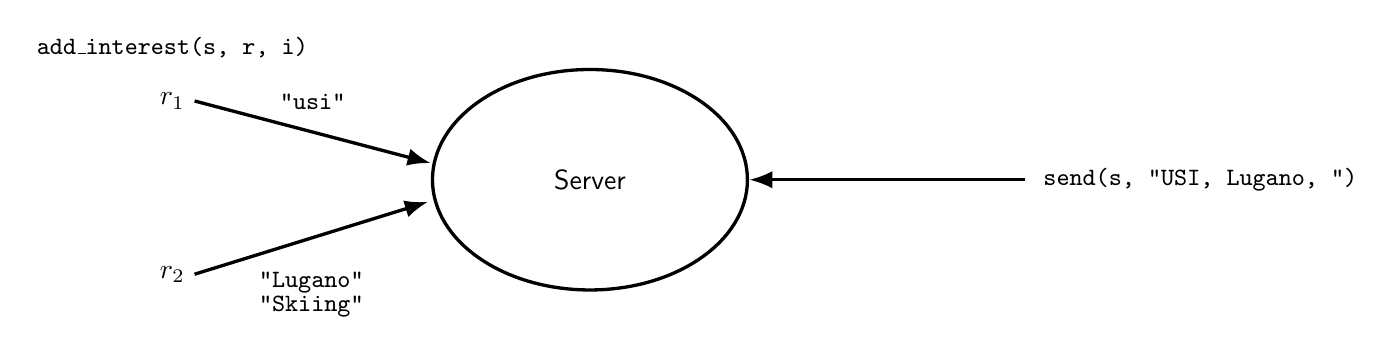
\begin{tikzpicture}[
  >=Latex,
  lbl/.style={font=\sffamily},
  code/.style={font=\ttfamily\small},
  every node/.style={lbl}
]

% Server node
\node[draw, ellipse, minimum width=40mm, minimum height=28mm, very thick] (server) {Server};

% Left side reference points
\node[left=30mm of server, yshift=10mm] (r1) {$r_1$};
\node[left=30mm of server, yshift=-12mm] (r2) {$r_2$};

% Arrow from r1 to server with midway label
\draw[->, very thick] (r1.east) -- ($(server.west)+(0,6pt)$)
  node[midway, above=1.5mm, code] {"usi"};

% Arrow from r2 to server with midway labels
\draw[->, very thick] (r2.east) -- ($(server.west)+(-1pt,-8pt)$)
  node[midway, below=3mm, code] {"Lugano"}
  node[midway, below=6mm, code] {"Skiing"};

% Outgoing arrow with label
\draw[<-, very thick] (server.east) -- ++(35mm,0)
  node[code, right=1mm] {send(s, "USI, Lugano, ")};

% Function label for add_interest
\node[code, above=2mm of r1] {add\_interest(s, r, i)};

\end{tikzpicture}
\end{document}